


\chapter{Machine Study Experiments}
\label{chap:machStudies}

\section{Introduction}

	Phase~I of BEAST~II occurred February 15 -- June 29 2016, during which the electron and positron beams were circulated in closed orbits around the SuperKEKB syncrotron but were not brought into collision. The rates in the \he tubes during Phase~I are shown in Fig \ref{fig:RateAll}.  In May, there were several periods of special machine experiments, where the beam conditions were set to study various background effects. These machine experiments included:  increasing the pressure of the gas in the beampipes, changing the size of the beams, varying the current in the beams, changing the size of the collimators in the beampipes, and studying the injection backgrounds.



\begin{figure}[htb]
	\centerfloat
		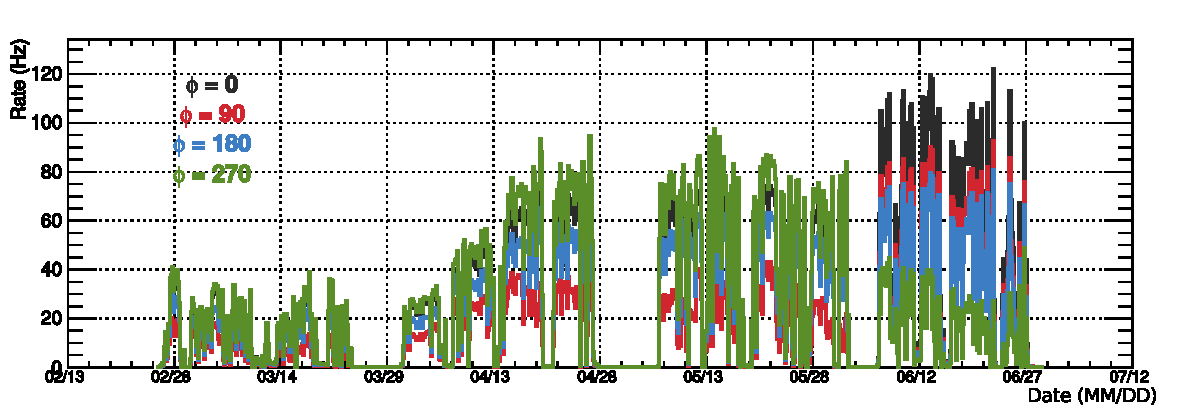
\includegraphics[trim={0 0 0 0.3cm},clip, width=\textwidth]{images/Rate_AllPhaseI}
	\caption[\He tube rates throughout BEAST~II Phase~I]{\He tube rates throughout BEAST~II Phase~I. The tubes located at $\phi=90$ and $\phi=270$ were swapped on June 1st.}	
	\label{fig:RateAll}
\end{figure}




\section{Pressure Experiments}


	To study the beam-gas interactions, the pressure in the beampipe was increased at various locations around the accelerator ring. These locations are shown in Fig \ref{fig:SKBVac}. Fig \ref{fig:VacuumBumpEg} shows an example of how the pressure at one of these locations changed with time.

\begin{figure}[htb]
	\centerfloat
		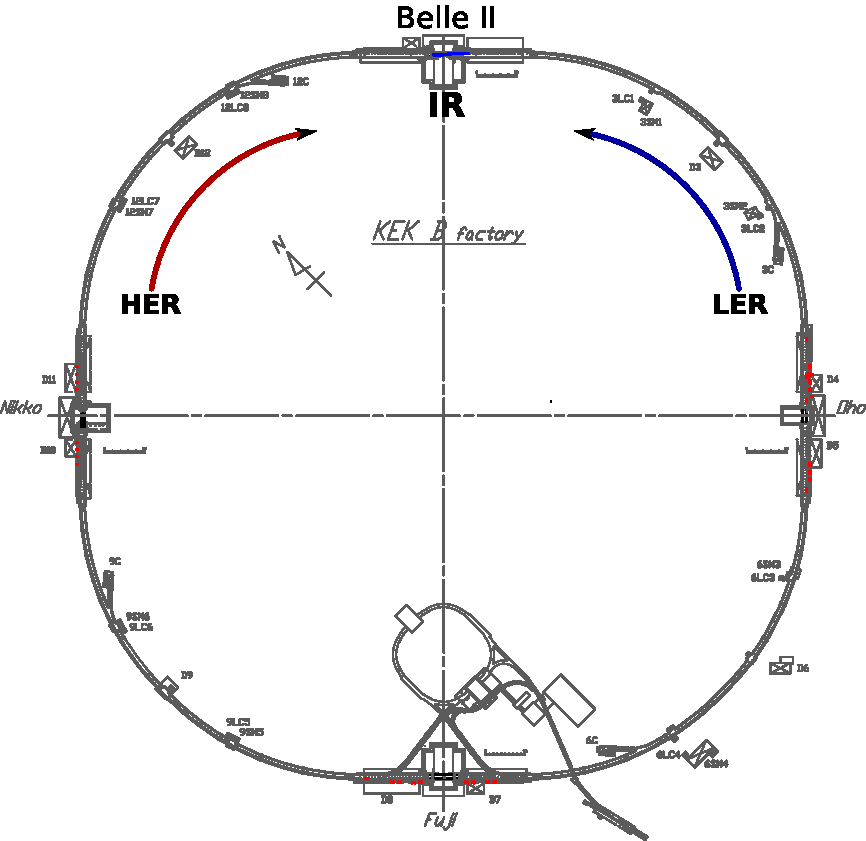
\includegraphics[scale=0.6]{images/SKEKb_key}

		\begin{picture}(2,2)
			\put(20,240){\color{blue}\thicklines\circle{20}}
			\put(110,135){\color{blue}\thicklines\circle{20}}
			\put(25,30){\color{blue}\thicklines\circle{20}}
			\put(-100,135){\color{blue}\thicklines\circle{20}}
	
			\put(80,210){\color{red}\thicklines\circle{20}}
			\put(-70,210){\color{red}\thicklines\circle{20}}
			\put(110,135){\color{red}\thicklines\circle{22}}
			\put(25,30){\color{red}\thicklines\circle{22}}
			\put(105,60){\color{red}\thicklines\circle{20}}
			\put(-70,60){\color{red}\thicklines\circle{20}}
		\end{picture}
	\caption[Locations of pressure increases]{Locations of pressure increases. LER locations are circled in blue, and HER locations are circled in red~\cite{SKBgroup}.}
	\label{fig:SKBVac}
\end{figure}

\begin{figure}[htb]
	\centerfloat
		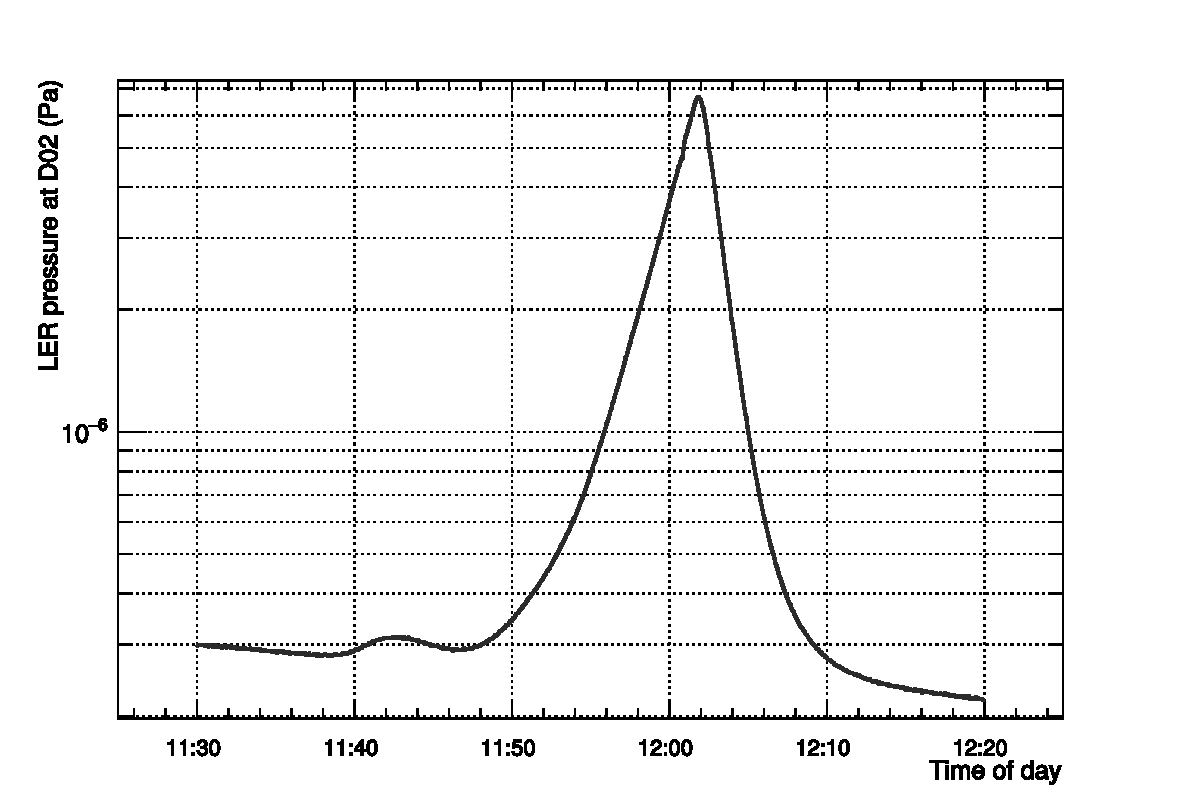
\includegraphics[trim={0 0 0 0.75cm},clip, width=\textwidth]{images/PressureBump}
	\caption[Example of pressure change during vacuum bump study]{Example of pressure change during vacuum bump study. Horizontal axis is log scale. Note the double bump. Data were recorded on May 23, 2016.}	
	\label{fig:VacuumBumpEg}
\end{figure}


	To reduce the beampipe pressure to an adequate vacuum level, Non-Evaporable Getter (NEG) pumps were used. These reduce the pressure by absorbing residual gas molecules in the beampipe. During the pressure bump studies, the NEGs at various locations around the beam were heated. This released the captured gas molecules back into the beampipe, increasing the pressure. The heating was done in two stages, which is the cause of the two bump structures seen in Fig \ref{fig:VacuumBumpEg}. 


\section{Touschek Experiments}



\begin{figure}[htb]
	\centerfloat
		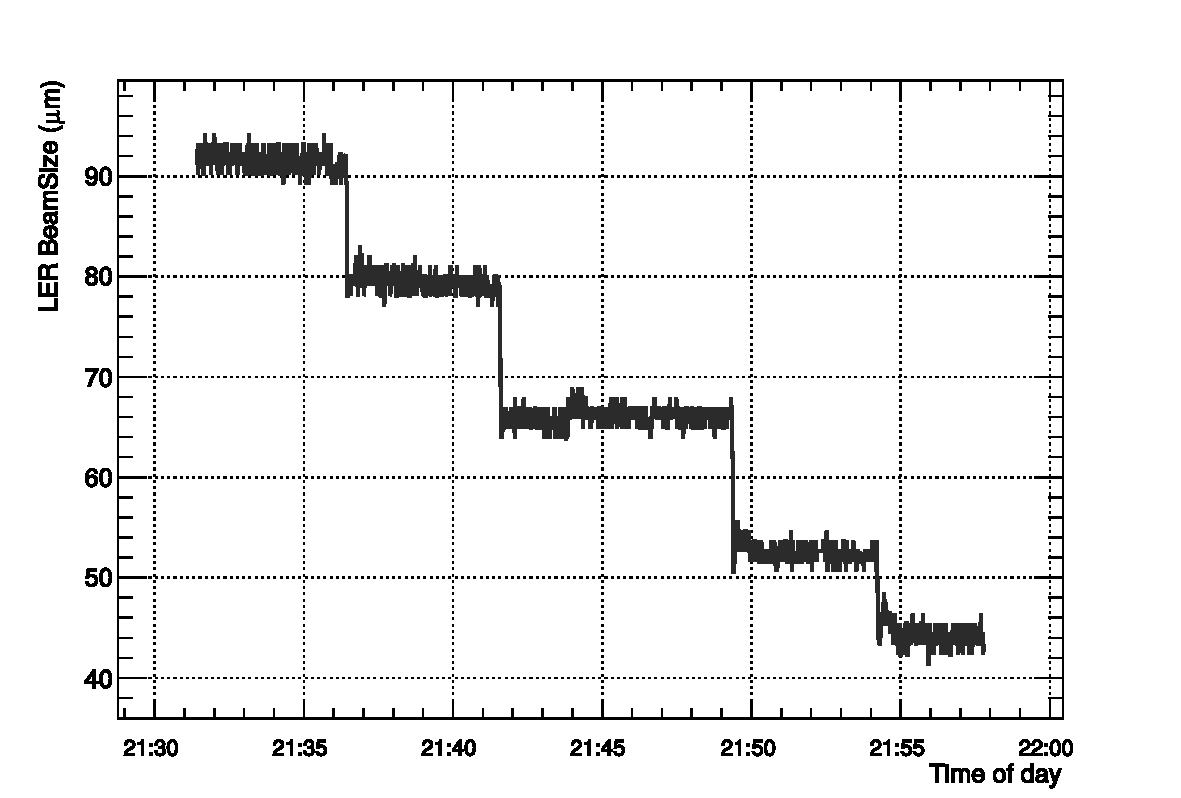
\includegraphics[trim={0 0 0 0.75cm},clip, width=\textwidth]{images/BeamSizeScan}
	\caption[Example of beam size change during beam size scan]{Example of beam size change during beam size scan. Data were recorded on May 17, 2016.}	
	\label{fig:BeamSizeEg}
\end{figure}


	To examine the Touschek contribution to the beam backgrounds, runs were taken where the size of the beam was varied. At each beam size setting, current was injected and allowed to decay over a period of time. An example of how the beam size changed during one of these runs is given in Fig \ref{fig:BeamSizeEg}.

	
	Different approaches were used to change the beam size in the LER and HER beams. In the LER, the x-y coupling of the beam was increased by changing the strength of some of the quadrupole magnets. This increased the vertical beam size without changing the beam orbit. This was attempted in the HER, but the change in beam size was not as dramatic as desired. Instead, the beam orbit at one of the bending magnets was adjusted, which increased the vertical dispersion and horizontal size. The beam orbit outside these bending magnets was unchanged~\cite{Hiro}.





\section{Vacuum Scrubbing}


	The beampipe walls contain gas molecules that were absorbed during manufacturing, shipping, etc. When beams are run through the beampipe, these molecules are desorbed from the surface of the beampipes by photons produced by the beams \cite{chao2013handbook}. Figure \ref{fig:LERPRECUR} shows the current and pressure in the LER beam as a function of time. When the LER current increases, the pressure also increases due to the desorption of gas molecules.

	As more beam is passed through the rings, there is less and less gas to be desorbed --- the beampipes get cleaner. This should manifest as a decrease in $dP/dI$, the change in pressure per change in current. This quantity is known as the dynamic pressure. The event rate measured in BEAST~II detectors should also decrease.



%	Most of Phase~I was vacuum scrubbing. In order to reduce the gas pressure in the beampipe, the particle beam is run with a large beam size. This causes the beampipe walls to expel the gas molecules they have absorbed. These gas molecules are then pumped out by the NEGs. 

%discussion of dP/dI


\begin{figure}[htb]
	\centerfloat
		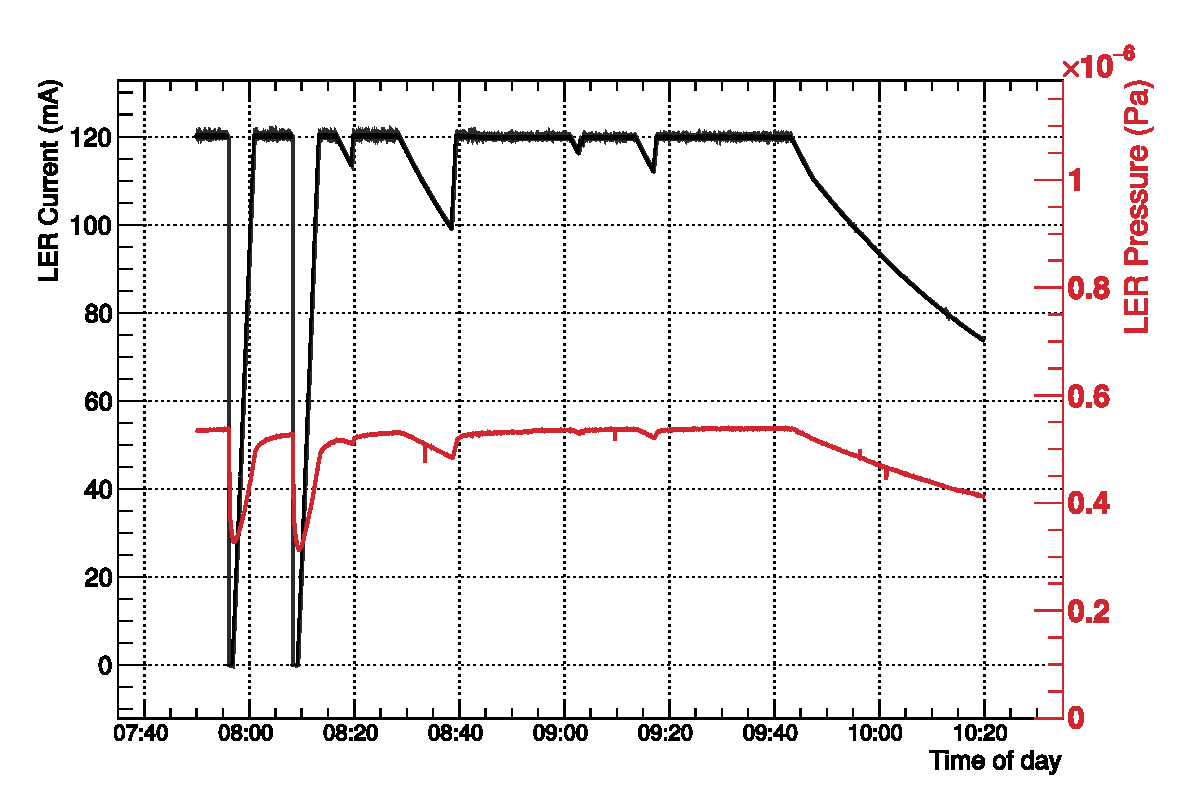
\includegraphics[trim={0 0 0 0.75cm},clip, width=\textwidth]{images/LER_PreAndCur}
	\caption[Example of LER current and pressure during vacuum scrubbing]{Example of LER current and pressure during vacuum scrubbing. When the beam current increases, the pressure increases too. Black is the beam current, and red is the beampipe pressure. Data were recorded on March 3, 2016.}
	\label{fig:LERPRECUR}
\end{figure}



\subsection{Analysis}


	During most of the vacuum scrubbing, both the HER and LER beams were running. In order to separate the effect of each beam, the average of the rates in the four \he tubes is fit to:
\begin{equation}
	{R_{^{3}\mathrm{He tube}} = A_{\mathrm{HER}} (P\cdot I)_{\mathrm{HER}}+A_{\mathrm{LER}} (P\cdot I)_{\mathrm{LER}}}
	\label{eqn:vacScrbModel}
\end{equation}
where $(P\cdot I)$ is the pressure times current for each beam. This model is very simple as it ignores any Touschek component, which is proportional to $I^2/(N_{\mathrm{Bunch}}\sigma_{y})$. During the scrubbing, the beam size was generally quite large, so the Touschek component would be small. Eqn \ref{eqn:vacScrbModel} can be be separated into the HER and LER components:
\begin{subequations}
\begin{align}
		{R_{\mathrm{HER}} = A_{\mathrm{HER}} (P\cdot I)_{\mathrm{HER}}} \\
		{R_{\mathrm{LER}} = A_{\mathrm{LER}} (P\cdot I)_{\mathrm{LER}}}
\end{align}
\end{subequations}
Figure \ref{fig:VacScrbExample} shows an example of this fit for one day of running.

\begin{figure}
	\centerfloat
		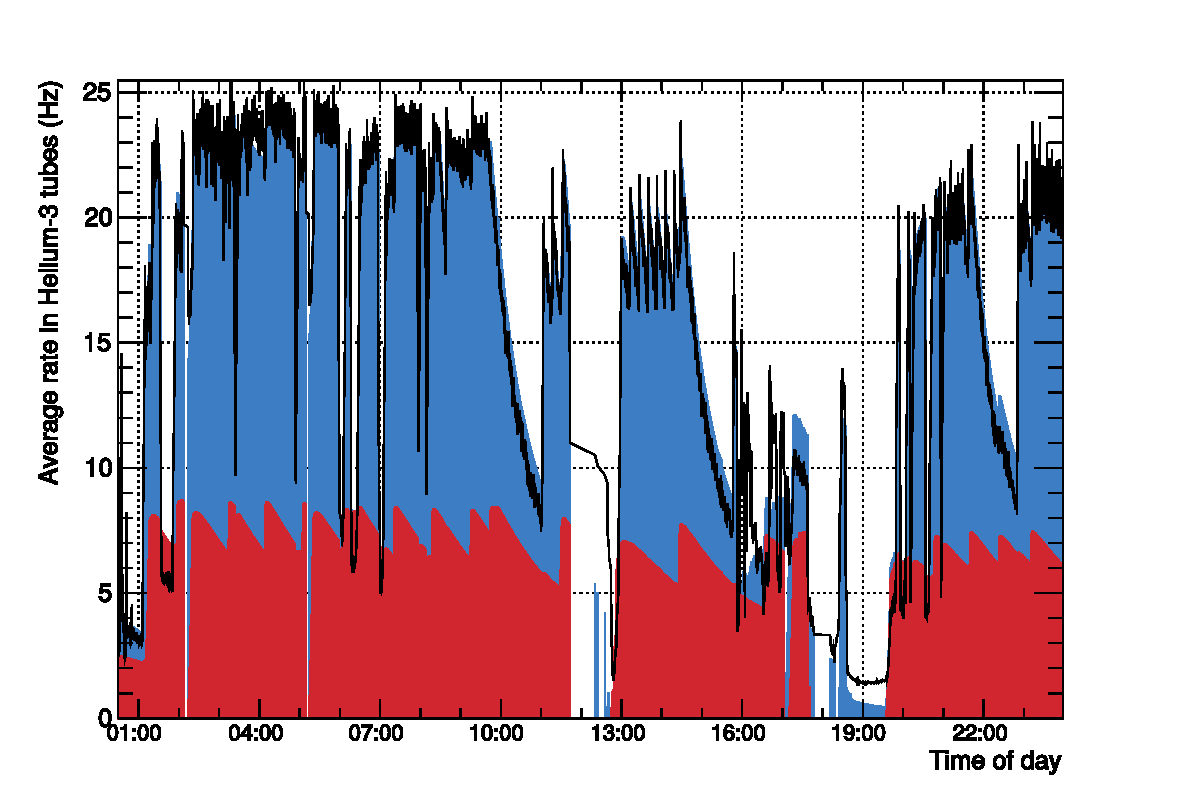
\includegraphics[trim={0 0 0 0.7cm},clip, width=\textwidth]{images/VacuumScrubFitExample}
	\caption[Fitting example for vacuum scrubbing]{Fitting example for vacuum scrubbing. Blue is the LER fit, red is the HER fit, and black is the average rate in the \he tubes. Data were recorded on March 3, 2016.}	
	\label{fig:VacScrbExample}
\end{figure}


The fit was recalculated for each day that data were taken. A requirement that both beams have at least 30 mA of current was applied. The rate was normalized by current squared. An average value of $R/I^2$ was calculated for each beam on each day of running, removing any days when the beams were off, or when the machine study experiments were being conducted. These daily values are plotted against the integrated current on the same day (see Fig \ref{fig:VacScrb}).

	The dynamic pressure $dP/dI$ as a function of the integrated current follows a power law of the form \cite{chao2013handbook}:
\begin{equation}
	{\frac{dP}{dI}\propto \left(\int{Idt}\right)^{-k}}
\end{equation}
$dP/dI$ is also plotted in Fig \ref{fig:VacScrb}, using data from \cite{SKBVacuum}. Both $R/I^2$ and dP/dI are fit to a power law, with the fit values shown in Table \ref{tab:PowerLawFits}. The parameters k for $R/I^2$ and $dP/dI$ are within 2$\sigma$ of each other, for both HER and LER, which shows that the effect of the vacuum scrubbing is observed with the \he tubes.


\begin{figure}
	\centering
	\subfigure[LER]{
		\begin{overpic}[trim={0 0 0 0.75cm},clip, width=\textwidth]{images/LER_withdPdI}
		\end{overpic}
		\label{fig:LERVacScrb}
	}
	\subfigure[HER]{
		\begin{overpic}[trim={0 0 0 0.75cm},clip, width=\textwidth]{images/HER_withdPdI}
		\end{overpic}
		\label{fig:HERVacScrb}
	}
	\caption[Vacuum scrubbing during BEAST~II Phase~I]{Vacuum scrubbing during BEAST~II Phase~I. Black is the dynamic pressure $dP/dI$ in each beam, and red or blue is the average rate of all four \he tubes, plotted against the integrated current. The \he tube follows the same trend as the dynamic pressure.}	
	\label{fig:VacScrb}
\end{figure}

\begin{table}
	\centering
	\begin{tabular}{ ccccc }
		&	\multicolumn{2}{c}{\He tubes}	& \multicolumn{2}{c}{$dP/dI$}					\\
  		& Constant (Hz/mA$^2$) 			& k		& Constant (Pa/mA) 		& k		\\\hline \hline
	LER	& (10.5$\pm$2)$\times10^{-3}$		& 0.81$\pm$0.04	& (16.9$\pm$2)$\times10^{-5}$	& 0.74$\pm$0.02	\\ 
	HER	& (8.0$\pm$1.4)$\times10^{-3}$		& 0.85$\pm$0.03	& (4.13$\pm$0.4)$\times10^{-5}$	& 0.89$\pm$0.02	\\ \hline

	\end{tabular}
	\caption[Power law fits for \he tube rate and $dP/dI$]{Power law fits for \he tube rate and $dP/dI$.}
	\label{tab:PowerLawFits}
\end{table}





























